\documentclass[12pt,twoside]{article}

% Things that are not loaded by the package, though these might be
% generally useful.
\usepackage{natbib}
\usepackage{graphicx}
\setcounter{secnumdepth}{0}

\usepackage{amsthm}

\renewcommand\thefigure{A.\arabic{figure}}
\renewcommand\thetable{A.\arabic{table}}
\renewcommand\theequation{A.\arabic{equation}}

% Load the package first - should sort everything out...
\usepackage{suppmat}

% ...and then we add some metadata
\titleprefix{Appendices}
\runninghead{Y fuse?}
\title{Y fuse? Sex chromosome fusions in fishes and reptiles}
\author{Matthew W. Pennell$^{\dag, 1,}$, Mark Kirkpatrick$^{\dag, 2}$, Sarah P. Otto$^{\dag, 3}$,\\ Jana C. Vamosi$^{4}$, Catherine L. Peichel$^5$, Nicole Valenzuela$^{6}$,\\ and Jun Kitano$^{7,*}$}
\address{
\dag& These authors contribued equally\\
1& Institute for Bioinformatics and Evolutionary Studies, University of Idaho, Moscow, ID 83844, USA\\
2& Department of Integrative Biology, University of Texas, Austin, TX 78712, USA\\
3& Department of Zoology, University of British Columbia, Vancouver, BC V6J 3S7, Canada\\
4& Department of Biological Sciences, University of Calgary, Calgary, AB T2N 1N4, Canada\\
5& Divison of Human Biology, Fred Hutchinson Cancer Research Center, Seattle, WA 98109, USA\\
6& Department of Ecology, Evolution and Organismal Biology, Iowa State University, Ames, IA 50011, USA\\
7& Ecological Genetics Laboratory, National Institute of Genetics, Mishima, Shizuoka 411-8540, Japan\\}
\emailaddress{*\email{jkitano@lab.nig.ac.jp}}
\date{}

\begin{document}

\maketitle


\section{Appendix 1: Theoretical analyses}

\subsection{Direct selection}

We track the rate of appearance and establishment of a sex-autosome fusion, where the rate at which mutation generates a fusion between a sex chromosome and an autosome is $\mu^{sex}_C$ per gamete per generation for chromosome $C$ ($C = X, Y, Z, \text{or} W$) in males ($sex = m$) and females ($sex = f$). We assume that, at birth, the population is of constant total size $N$, consisting of an equal number ($N/\text{2}$) of males and females. Not all individuals survive and successfully enter the reproductive pool. Specifically, we assume that the numbers of females and males that reproduce are $N^f$ and $N^m$, where each of these reproductive individuals is expected to have a Poisson distributed number of offspring. The effective population sizes of Y and W chromosomes are then $N_{e,Y}=N^m$ and $N_{e,W}=N^f$, respectively, while the effective population sizes of X and Z chromosomes equal:
\begin{subequations}
\begin{equation}
N_{e,X} = \frac{\text{9}N^fN^m}{N^f + \text{2}N^m}
\end{equation}
\begin{equation}
N_{e,Z} = \frac{\text{9}N^fN^m}{\text{2}N^f + N^m}
\end{equation}
\end{subequations}
(\citealt{Wright1933}; see also \citealt{Caballero1995} for extensions to non-Poisson distributions). Note that the above equations define the effective number of chromosomes, not the effective number of individuals.

Once the fusion appears, we approximate its establishment rate using Kimura's \citeyearpar{Kimura1962} diffusion approximation for the fixation probability. In the supplemental \emph{Mathematica} notebook, we allow for arbitrary levels of dominance of the fusion (including underdominance). Dominance has little effect on which type of fusion is expected to become established most frequently. Hence, we focus here on the simpler additive case, where the fixation probability of a fusion is:
\begin{equation}\label{eq:pc}
P_C = \frac{\text{1} - \exp[-\text{2}s_C N_{e,C}p]}{\text{1} - \exp[-\text{2}N_{e,C}s_C ]}
\end{equation}
where $s_C$ is the selection coefficient acting directly upon individuals carrying the fusion when rare (as heterozygotes), $p$ is the initial frequency of the fusion, and $N_{e,C}$ is the relevant effective population size of the chromosome $C$. (Recall that $N_{e,C}$ is the effective number of chromosomes, not individuals, which is why `\text{2}' rather than the standard `\text{4}' appears in Equation \ref{eq:pc}.) We also assume that selection on the fusion is sufficiently weak that the selection coefficient can be taken as the average over many generations, accounting for the time spent in each sex:
\begin{subequations}
\begin{equation}
s_X = \frac{\text{2}}{\text{3}}s^f_X + \frac{\text{1}}{\text{3}}s^m_X
\end{equation}
\begin{equation}
s_Y = s^m_Y
\end{equation}
\begin{equation}
s_Z = \frac{\text{1}}{\text{3}}s^f_Z + \frac{\text{2}}{\text{3}}s^m_Z
\end{equation}
\begin{equation}
s_W = s^f_W
\end{equation}
\end{subequations}
Below, we consider both the rate at which fusions originate and the rate at which they fix, for fusions involving different sex chromosomes.

\subsubsection{Y-A fusions}

Y-A fusions appear in the population at rate $\frac{N}{\text{2}}\mu^m_Y$. The probability that the fusion fixes is the chance that the fusion contributes to the reproductive population size of males in that generation, $N^m / (N/\text{2})$, times the probability that the fusion will be the ultimate ancestor of the Y chromosomes among the descendants after some long period of time, given by (\ref{eq:pc}) for the $C = Y$ chromosome with $N_{e,Y}=N^m$ and $p=\text{1}/N^m$. Multiplying the mutation rate by the fixation probability, the overall establishment probability for a Y-A fusion is
\begin{align}\label{eq:Ry}
R_Y &= N^m \mu^m_Y  P_Y \nonumber \\
&= N^m \mu^m_Y \frac{\text{1}-\exp[-\text{2}s_Y]}{\text{1}-\exp[-\text{2}N^ms_Y]}
\end{align}

\subsubsection{X-A fusions}

X-A fusions appear in the population at rate $\frac{N}{\text{2}}\mu^f_X$ among females and at rate $\frac{N}{\text{2}}\mu^m_X$ among males, where the former expression accounts for the fact that females carry two X chromosomes. A fusion arising in a female has a chance $N^f/\frac{N}{\text{2}}$ of surviving to reproduce. The probability that the fusion will be the ultimate ancestor of the X chromosomes after some long period of time is then given by (\ref{eq:pc}) for $C = X$, with $N_{e,X}$ given by (A.\text{1}a) and $p=\frac{\text{2}}{\text{3}}/(\text{2}N^f)$ accounting for the fact that $\frac{\text{2}}{\text{3}}$ of the X chromosomes in the next generation come from these mothers, among whom the fusion is at initial frequency $\text{1}/(\text{2}N^f)$. A similar calculation applies to males, so that the net establishment rate is approximately:
\begin{equation}\label{eq:Rx}
R_X = \text{2}N^f\mu^f_X 
\frac{\text{1}- \exp[-\text{2}s_X N_{e,X}  \frac{\text{2}}{\text{3}} \frac{\text{1}}{\text{2}N^f} ]}{\text{1} - \exp[-\text{2}N_{e,X} s_X]} 
+ \text{2}N^m\mu^m_X \frac{\text{1}- \exp[-\text{2}s_X N_{e,X}  \frac{\text{1}}{\text{3}} \frac{\text{1}}{N^m}]}{\text{1} - \exp[-\text{2}N_{e,X} s_X]}
\end{equation}

\subsubsection{W-A fusions}
The establishment rate of W-A fusions, $R_W$, is derived as for Y-A fusions, giving (\ref{eq:Ry}) but with $m$ replaced by $f$ and $Y$ replaced by $W$.

\subsubsection{Z-A fusions}
The establishment rate of Z-A fusions, $R_Z$, is derived as for X-A fusions, giving (\ref{eq:Rx}) but with $m$ and $f$ interchanged and $X$ replaced by $Z$.

\subsubsection{Neutral fusions}
When selection is negligible, the above formulae can be simplified substantially. In the limit for neutral fusions ($s_C=\text{0}$), the net establishment rate equals the rate at which each type of fusion arises: 
\begin{subequations}
\begin{equation}
R_Y=\mu_Y,
\end{equation}
\begin{equation}
R_X=\frac{\text{2}}{\text{3}}\mu^f_X + \frac{\text{1}}{\text{3}}\mu^m_X,
\end{equation}
\begin{equation}
R_W=\mu_W,
\end{equation}
\begin{equation}
R_Z=\frac{\text{2}}{\text{3}}\mu^m_Z + \frac{\text{1}}{\text{3}}\mu^f_Z.
\end{equation}
\end{subequations}
Observe that the reproductive population sizes of males ($N^m$) and females ($N^f$) are irrelevant to the relative rate of fusion establishment when there is no direct selection on the fusions. A neutral fusion is less likely to survive and reproduce if it first appears in the sex with the lower reproductive population size, but if it does, then it has a higher chance of being the progenitor chromosome; these effects exactly cancel out.

\subsubsection{Weak selection}

The relative establishment rates also get simplified substantially when selection is very weak: $|\theta| << \text{1}$, where $\theta=\text{4}Ns_C$. To leading order in $\theta$, the establishment rate for each type of fusion, measured relative to the rate of X-A fusions, is:
\begin{subequations}
\begin{equation}
\frac{R_Y}{R_X} = \frac{\text{3}\beta}{\text{2} +\beta} \left(\text{1} + \theta \frac{\text{1} - \text{4}\gamma}{\text{4}\gamma(\text{2}+\gamma)} \right),
\end{equation}
\begin{equation}
\frac{R_W}{R_X} = \frac{\text{3}}{\text{2} +\beta} \left(\text{1} - \theta \frac{\text{7} - \gamma}{\text{8}(\text{2}+\gamma)} \right),
\end{equation}
\begin{equation}
\frac{R_Z}{R_X} = \frac{\text{2}\beta + \text{1}}{\text{2} +\beta} \left(\text{1} + \theta \frac{\text{9}(\text{1} - \gamma)}{\text{8}(\text{2}+\gamma)(\text{1}+\text{2}\gamma)} \right),
\end{equation}
\end{subequations}
where fusions arise in males at a rate $\beta=\mu^m/\mu^f$ times that in females and the number of reproductive females is $\gamma=N^f/N^m$ times the number of males (so that the sex ratio $N^m/(N^m + N^f) = \text{1}/(\gamma + 1)$). In the absence of a sex bias in the mutation rate ($\beta=\text{1}$) or number of reproductive individuals ($\gamma=\text{1}$), we find that 
\[\frac{R_Y}{R_X}=\frac{R_W}{R_X}=\text{1} - \frac{\theta}{\text{4}} \]
and 
\[\frac{R_Z}{R_X} = \text{1}.\]
This confirms that direct selection alone cannot explain the predominance of Y-A fusions. 

Similarly, the overall rate at which fusions arise in XY systems versus ZW systems is the sum of the rates for the component chromosomes, keeping only leading order terms in $\theta$:
\begin{align}
\frac{R_X + R_Y}{R_Z + R_W} &= \frac{\text{1}+\text{2}\beta}{\beta + \text{2}} 
+ \frac{\theta}{\text{2}} \left[ \left(\frac{\text{3}\beta}{\text{2} + \beta} \right)
\left(\frac{\text{1}-\text{4}\gamma}{\text{4}\gamma(\text{2}+\gamma)}\right) +  \right. \nonumber \\
&\qquad \left.
\left(\frac{\text{3}(\text{1}+\text{2}\beta)}{(\text{2}+\beta)^\text{2})} \right)
\left(\frac{\text{7}-\gamma}{\text{8}(\text{2}+\gamma)} \right) - 
\left(\frac{(\text{1}+\text{2}\beta)^\text{2}}{(\text{2}+\beta)^\text{2})} \right)
\left(\frac{\text{9}(\text{1}-\gamma)}{\text{8}(\text{2}+\gamma)(\text{1}+\text{2}\gamma)} \right) \right].
\end{align}

\subsection{Sex-Antagonistic selection}
Consider an autosomal locus with selection acting in opposite directions in males and females, with allele $A_0$ favored in males and allele $A_\text{1}$ in females. If selection is weak, the allele frequency $q_i$ of allele $A_i$ is approximately the same in males and females. Given the sex-specific fitness of genotype $ij$, $W^{sex}_{ij}$, we can then define the selection coefficient favoring allele $A_i$ in a particular sex as $s^{sex}_i=(W^{sex}_{i.}/\bar{W}^{sex})-\text{1}$. Here $W^{sex}_{i.}$ is the marginal fitness of $A_i$ in that sex ($W^{sex}_{i.}=q_0W^{sex}_{i0} + q_\text{1}W^{sex}_{i\text{1}}$), and $\bar{W}^{sex}$ is the mean fitness ($\bar{W}^{sex} = q_0W_{0.} + q_1W_{1.}$).

Following similar logic used to derive equations (A.4) and (A.5), fusions bearing allele $A_i$ arise with the Y chromosome and are found in a reproductive male at rate $q_i\mu^m_YN^m$  or arise with the W and are found in a reproductive female at rate $q_i\mu^f_WN^f$. Similarly, the rate at which X-A fusions or Z-A fusions bearing allele $A_i$ originate is $q_i(\text{2}\mu^f_XN^f + \mu^m_XN^m)$ or $q_i(\mu^f_ZN^f + \text{2}\mu^m_ZN^m)$, respectively. If we assume selection is weak, we can average over the time the chromosome spends in a female and a male to obtain the strength of selection acting on a fusion bearing allele $A_i$: $s_{X,i}=\frac{\text{2}}{\text{3}}s^f_i + \frac{\text{1}}{\text{3}}s^m_i$ for an X-A fusion, $s_{Y,i}=s^m_i$ for a Y-A fusion, $s_{Z,i}=\frac{\text{1}}{\text{3}}s^f_i + \frac{\text{2}}{\text{3}}s^m_i$  for a Z-A fusion, and $s_{W,i}=s^f_i$ for a W-A fusion.
 
Because the X and W are more often found in females, the fixation probability of an X-A or W-A fusion is much higher if it captures the female-benefit allele A\text{1} than if it captures the male-benefit allele (and \emph{vice versa} for Y-A and Z-A fusions). Using $\text{2}s_CN_{e,C}p$ to approximate the fixation probability (A.\text{2}) for a beneficial fusion initially at frequency $p$, the fixation probability of an X-A fusion is approximately $P_{X}=\text{2}s_{X,\text{1}}N_{e,X}p$ when it captures allele $A_\text{1}$ and zero otherwise. Similarly, $P_W = \text{2}s_{w,\text{1}}N_{e,W}p$ when a W-A fusion captures $A_\text{1}$, $P_Y = \text{2}s_{Y,0}N_{e,Y}p$ when a Y-A fusion captures $A_0$, and $P_Z=\text{2}s_{Z,0}N_{e,Z}p$ when a Z-A fusion captures $A_0$.

Multiplying together the rate that fusions originate in each sex times their fixation probability (accounting for the initial frequency in that sex), we get the rate at which fusions are expected to become established for each sex chromosome:
\begin{subequations}
\begin{equation}
R_Y = q_0 \mu_Y N^m \text{2}s^m_0,
\end{equation}
\begin{equation}
R_X = \text{2} q_\text{1} \frac{9N^fN^m}{N^f + \text{2}N^m} 
\left( \frac{\text{2}}{\text{3}}\mu^f_X + \frac{\text{1}}{\text{3}}\mu^m_X \right)
\left( \frac{\text{2}}{\text{3}}s^f_\text{1} + \frac{\text{1}}{\text{3}}s^m_\text{1} \right),
\end{equation}
\begin{equation}
R_W = q_\text{1} \mu_W N^f \text{2}s^f_\text{1},
\end{equation}
\begin{equation}
R_z = \text{2} q_0 \frac{9N^fN^m}{N^f + \text{2}N^m} 
\left( \frac{\text{1}}{\text{3}}\mu^f_Z + \frac{\text{2}}{\text{3}}\mu^m_Z \right)
\left( \frac{\text{1}}{\text{3}}s^f_0 + \frac{\text{2}}{\text{3}}s^m_0 \right).
\end{equation}
\end{subequations}

At an autosomal locus subject to sexually antagonistic selection, each allele has spent half of its time in males and half in females, rising in frequency in one sex and falling in the other sex. Consequently, to remain at equilibrium over the longer term, the selection coefficients for each allele must balance across the sexes, with $s^f_0 = -s^m_0$ and $s^f_\text{1} = -s^m_\text{1}$ (see formal proof in the supplemental \emph{Mathematica} notebook). Furthermore, the fitness definitions imply that $q_0s^{sex}_0 + q_\text{1}s^{sex}_\text{1}$ must equal zero since they sum to
\[\frac{q_0W^{sex}_{0.} + q_\text{1}W^{sex}_{\text{1}.}}{\bar{W}^{sex}} - \text{1} = \frac{\bar{W}^{sex}}{\bar{W}^{sex}} - \text{1} = 0.\]
Using these relationships to substitute for $s^f_i$ and $q_\text{1}$, we find:
\begin{subequations}
\begin{equation}
R_Y = \text{2}s^m_0 q_0 (\mu_YN^m),
\end{equation}
\begin{equation}
R_X = \text{2}s^m_0 q_0 \left(\frac{(\text{2}\mu^f_X + \mu^m_X)N^fN^m}{N^f + \text{2}N^m} \right),
\end{equation}
\begin{equation}
R_W = \text{2}s^m_0 q_0 (\mu_WN^f),
\end{equation}
\begin{equation}
R_Z = \text{2}s^m_0 q_0 \left(\frac{(\mu^f_Z + \text{2}\mu^f_Z)N^fN^m}{N^f + \text{2}N^m} \right).
\end{equation}
\end{subequations}
Thus, with equal mutation rates and equal numbers of reproductive individuals of the two sexes, the establishment rates all equal one another. Otherwise, recalling that $\beta = \mu^m/\mu^f$ and $\gamma = N^f / N^m$, the establishment rates relative to the rate of X-A fusions become:
\begin{subequations}
\begin{equation}
\frac{R_Y}{R_X} \approx \frac{\beta(\text{2} + \gamma)}{\gamma(\text{2} + \beta)},
\end{equation}
\begin{equation}
\frac{R_W}{R_X} = \frac{\text{2} + \gamma}{\text{2} + \beta},
\end{equation}
\begin{equation}
\frac{R_Z}{R_X} = \frac{(\text{1} + \text{2}\beta)(\text{2} + \gamma)}{(\text{1} + \text{2}\gamma)(\text{2} + \beta)},
\end{equation}
\end{subequations}
Consequently, Y-A fusions are expected to predominate if and only if $\beta > \gamma$.

\section{Appendix 2: Details of phylogenetic analyses}

To investigate the relative rates of different types of fusions across our two focal groups--teleost fishes and squamate reptiles--we fit multiple phylogenetic models to our karyotype dataset. We first matched the available karyotype data to the fish \citep{Rabosky2013} and squamate \citep{squamatetree, PyronBurbrink2014} phylogenies (using an approximate matching algorithm described in the main text). This resulted in phylogenetic comparative datasets containing 163 species of fish and 261 squamate species.  We conducted two separate types of analyses on both groups. First, we examined differences between XY and ZW systems; here, we treat X-autosome and Y-autosome fusions as equivalent (see below), and likewise, Z-autosome and W-autosome fusions. Results from this first analysis are presented in the main text. Second, we investigated autosomal fusion rates for all types of sex chromosomes individually (i.e., Y-, X-, W-, and Z-autosome fusions). While the second analysis provides more detailed resolution, some of the states are rarely observed (and in some cases, not at all). All analyses were performed using the R package \textsc{diversitree} \citep{FitzJohn2012}, and code to reproduce all results can be found at \texttt{https://github.com/mwpennell/fuse/analysis}. 

\subsection{Fusion rates in XY vs. ZW systems}

Using a Markov model \citep{Pagel1994}, we considered transitions among the following states:
\begin{itemize}
\item $XY$: Male heterogametic unfused
\item $XY_F$: Male heterogametic fused (XXY or XYY)
\item $ZW$: Female heterogametic unfused
\item $ZW_F$: Female heterogametic fused (ZZW or ZWW)
\end{itemize}
allowing transitions between all states with $q_{A.B}$ representing the transition rate between states $A$ and $B$. We then used likelihood ratio tests to restrict the model in order to improve our ability to estimate the parameters of interest. 

We first imposed the biologically reasonable constraint that prior to becoming $XY_F$ (or $ZW_F$), a lineage must first be $XY$ (or $ZW$); e.g., the transition rate from female heterogametic unfused to male heterogametic fused $q_{ZW.XY_F}$ would be zero. These restrictions did not lead to a significant decline in likelihood for either squamates or fish and was accepted.

Next, we proposed a model in which the rate of switching the heterogametic sex, going from a XY to a ZW system and \emph{vice versa}, did not depend on whether the lineage contained a fused sex chromosome or not (e.g., $q_{XY_F.ZW} = q_{XY.ZW}$). In both fish and squamtes, this restriction was acceptable using likelihood ratio tests.

In the next step, we proposed a model in which the rate of chromosomal fission, going from a fused sex chromosome system to an unfused system of the same type, was the same for XY and ZW systems. In fish, a likelihood ratio test favored the more restricted model, whereas in squamates, the more general model (where $q_{XY_F.XY} \neq q_{ZW_F.ZW}$) was favored ($p=\text{0.012}$). The support for the more general model in squamates stems from the scarcity of ZW fusions in the data; there is little information to reliably estimate the transition rate from fused female heterogametic to unfused female heterogametic ($q_{ZW_F.ZW}$) using maximum likelihood (see below). We therefore took slightly different approaches when analyzing the two clades.

For fish, we compared the resulting model ($q_{XY_F.XY} = q_{ZW_F.ZW}, q_{ZW.XY_F}=q_{XY.ZW_F}=\text{0}, q_{XY_F.ZW}=q_{XY_Z.ZW}, q_{ZW_F.XY}=q_{ZW.XY}$) to an even more reduced model in which the XY and ZW fusion rates were set to be equal ($q_{XY.XY_F}=q_{ZW.ZW_F}$). We found the rate difference to be highly significant ($p=\text{0.014}$) using a likelihood ratio test. To better accomodate uncertainty in the estimate, we ran a Bayesian analysis (described in the text), and this too supported our conclusion that XY fusions occur at a higher rate than ZW fusions (98.6\% of the posterior probability supported this and the 95\% credibility interval for the difference in rates did not overlap with zero; Figure 4 in the main text).

For the squamate data, we took two approaches. First, we assumed that the `equal fission rates model' was indeed reasonable and performed the same analysis as in fish. Using a likelihood ratio test, the difference in fusion rates for XY and ZW was found to be highly significant ($p=\text{0.003}$). The same was true for the Bayesian analysis (99.9\% of the posterior probability distribution supported this conclusion; Figure 4 in the main text). Second, we used a Bayesian MCMC to fit a model in which the fission rate $q_{ZW_F.ZW}$ was estimated independently of $q_{XY_F.XY}$. For this model the support for the difference between XY and ZW fusion rates was not as strong (92.0\% of the posterior probability supported $q_{XY.XY_F} > q_{ZW.ZW_F}$; Figure \ref{fig:squa-dif}).

\begin{figure}[p]
\centering
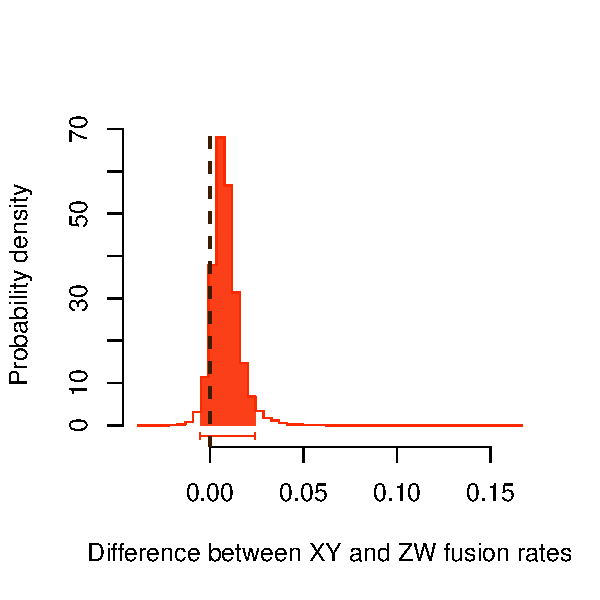
\includegraphics[scale=1.25]{figs/karyotype-fusion-squa-6par}
\caption{Posterior estimate of the rate difference between XY and ZW fusions ($q_{XY.XY_F} - q_{ZW.ZW_F}$) in squamate reptiles when we allow the fission rates $q_{XY_F.XY}$ and $q_{ZW_F.ZW}$ to differ.}
\label{fig:squa-dif}
\end{figure}

As mentioned above, the squamate data contain very little information about fission rates, especially from $ZW_F$ to $ZW$. The likelihood approach has difficulty distinguishing between two explanations for the lack of fused ZW chromosomes: rare ZW fusions or common ZW fissions. Nevertheless, there is a strong signal that ZW fusions should be less common, which we confirmed by considering residency times $t_R$, the average evolutionary duration of a fused state. For XY fusions,
\begin{equation}
t_{R,XY_F} = \frac{q_{XY.XY_F}}{q_{XY.XY_F} + q_{XY_F.XY}}
\end{equation}
and for ZW fusions
\begin{equation}
t_{R,ZW_F} = \frac{q_{ZW.ZW_F}}{q_{ZW.ZW_F} + q_{ZW_F.ZW}}
\end{equation}
Using a Bayesian analysis, we found very strong support for the residency time being greater for XY fusions than ZW fusions (99.8\% of the posterior probability supported $t_{R,XY_F} > t_{R,ZW_F}$; Figure \ref{fig:squa-resid}). In the absence of direct information about fission rates for fused ZW chromosomes, we conclude that the data is more parsimoniously explained by rare ZW fusions, while acknowledging that rapid ZW fission rates may also explain the data for squamates.

\begin{figure}[p]
\centering
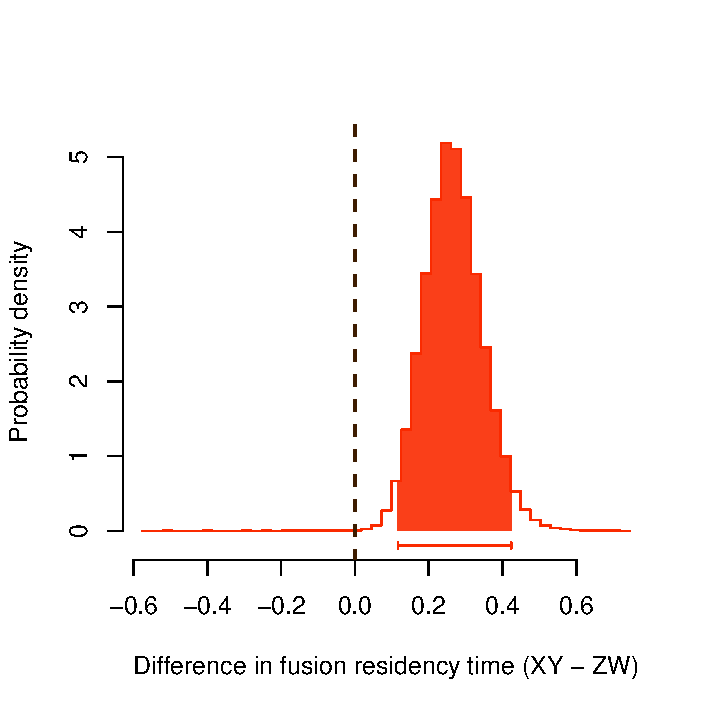
\includegraphics[scale=1.1]{figs/karyotype-residency-squa-6par}
\caption{Posterior estimate of the difference in residency time between XY and ZW fusions (i.e., $t_{R,XY_F} - t_{R,ZW_F}$) in squamate reptiles.}
\label{fig:squa-resid}
\end{figure}


\subsection{Comparing fusion rates between chromosomes} 

Rather than classifying the states as male/female heterogametic unfused/fused, we separated out the different types of fusions (e.g., classifying X-autosome [XA] and Y-autosome [YA] fusions as different states). This allowed us to assess whether the patterns we observed were driven by an overabundance of autosomal fusions with the Y chromosome. After matching the data to the tree, we did not have any records of WA fusions in fish while in squamates, XA fusions were absent. We thus considered models with only three fused states (for fish: XA, YA, and ZA; for squamates: YA, WA, and ZA)

For both the fish and the squamates, we again restricted the model via a nested series of likelihood ratio tests. For both clades, we found it to be statistically justifiable to assume that: a) transitions from one fused state directly to another fused state were impossible; b) prior to becoming fused, a lineage had to be in the corresponding unfused state; and c) fission rates were constrained to be equal. This allowed us to reliably evaluate whether the fusion rates differed by chromosome.

For the fish, using likelihood ratio tests, we found YA fusions to be significantly higher than XA fusions ($p=\text{0.016}$) and ZA fusions ($p=\text{0.035}$), but that XA and ZA fusion rates were not significantly different ($p=\text{0.658}$). Again, WA fusions did not exist in the fish analysis so we could not compare them to other classes. We then performed a Bayesian MCMC analysis to gain a better estimate of the relevant parameters. For the purposes of this analysis, we fixed XA and ZA fusions to occur at the same rate and then compared this rate to that for YA fusion. We found that YA fusions occur at a much higher rate than XA/ZA fusions (Figure \ref{fig:fish-ind}; 99.5\% of the posterior distribution supported this conclusion).

\begin{figure}[p]
\centering
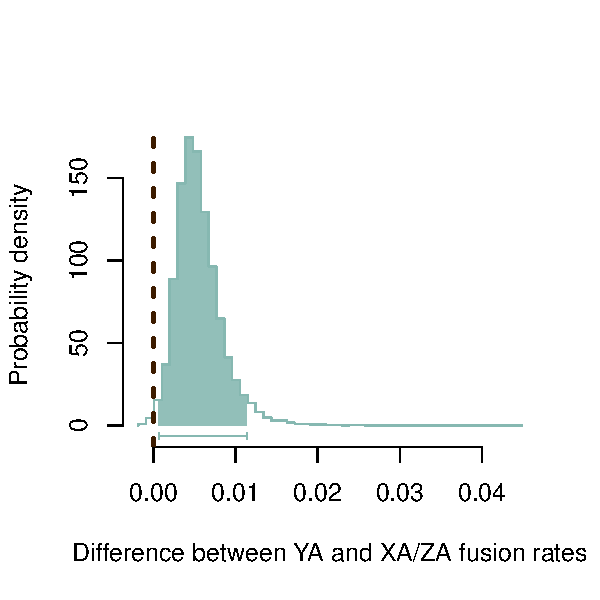
\includegraphics[scale=1.25]{figs/chromosome-fusion-fish}
\caption{Posterior estimate of the rate difference between YA and XA/ZA fusions in fish. When the estimate is greater than zero, this means that the YA fusion rates are higher than those of the other chromosomes}
\label{fig:fish-ind}
\end{figure}

For the squamate analysis, YA fusions also occured at a higher rate than WA fusions ($p<\text{0.001}$) and ZA fusions ($p<\text{0.001}$). WA and ZA fusions rates were not significantly different from one another ($p\approx \text{1}$). As with the fish, for the Bayesian analysis we set WA and ZA fusion rates to be equal and estimated the difference between YA fusions and other type of fusions. 99.9\% of the posterior probability distribution supported YA fusions occuring at a higher rate than fusions on other chromosomes (Figure \ref{fig:squa-ind}). 

Taken together, these results strongly suggest that the difference between XY and ZW fusion rates is driven almost entirely by the very high rates of autosomal fusions involving the Y chromosome relative to the other sex chromosomes.

\begin{figure}[p]
\centering
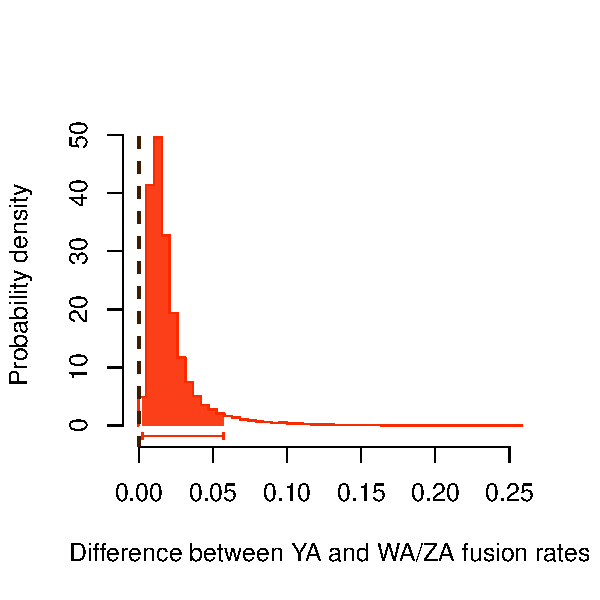
\includegraphics[scale=1.25]{figs/chromosome-fusion-squa}
\caption{Posterior estimate of the rate difference between YA and WA/ZA fusions in squamate reptiles. When the estimate is greater than zero, this means that the YA fusion rates are higher than those of the other chromosomes}
\label{fig:squa-ind}
\end{figure}

\clearpage
\bibliographystyle{sysbio}
\bibliography{suppmat.bib}

\end{document}
